\documentclass{article}
\usepackage{graphicx} % Required for inserting images
\usepackage{amsmath} 
\usepackage{amssymb}
\usepackage{multicol} % For multicols environment
\usepackage{color}
\usepackage[dvipsnames]{xcolor}
\usepackage{pdflscape}
\pagenumbering{gobble} % Remove os números de página
\usepackage[left=0.5cm,
            right=0.5cm,
            top=1cm,
            bottom=0.5cm]{geometry}
\usepackage{tikz}
\usepackage{amsmath, amsfonts, amssymb, amsthm, tikz-cd, multicol, nccmath, mathtools, graphicx}
\usetikzlibrary{decorations.pathmorphing}

\newcommand{\boxedpic}[2]{% #1 = título, #2 = conteúdo tikz
  \begin{center}
    \begin{minipage}{0.8\linewidth}
      \centering
      \textbf{#1}\\[0.5ex]
      #2
    \end{minipage}
  \end{center}
  \vspace{1em}
}
\title{Colinha}


\definecolor{cinza}{gray}{0.85}

\begin{document}
\begin{landscape}

\begin{multicols}{3}

\section{Bases}

\textbf{Def.}: $(X, \tau)$ esp. top. Dizemos que $\mathcal{B} \subset \tau$ é uma \underline{base} p/ $(X, \tau)$ se p/ todo aberto não vazio $A \in \tau$, existe uma família $\mathcal{A} \subset \mathcal{B}$ de elementos da base t.q. $A = \bigcup_{B \in \mathcal{A}}B$.\\
\textbf{Prop.}: Uma família $\mathcal{B}$ de elementos de $\tau$ é uma base p/ $(X, \tau) \iff$ p/ todo aberto não vazio $A \in \tau$ e todo $x \in A, \exists B \in \mathcal{B}$ de forma que $x \in B \subset A$.\\
\textbf{Exemplo}: $\mathcal{B} = \{]a,b[: a,b \in \mathbb{Q}\}$ é uma base p/ a topologia usual de $\mathbb{R}$.\\
\textbf{Exemplo}: Seja $X$ um conjunto qualquer. $\mathcal{B} = \{\{x\} : x \in X\}$ é uma base p/ a topologia discreta sobre $X$.\\
\textbf{Def.}: $(X, \tau)$ esp. top. $x \in X$. Dizemos que $\mathcal{V}$ é um \underline{sistema fundamental de vizinhanças} (s.f.v) de $x$ se:\\
a) $\forall V \in \mathcal{V}$, $V$ é vizinhança de $x$;\\
b) $\forall A \subset X$ aberto t.q. $x \in A, \exists V \in \mathcal{V}$ t.q. $x \in V \subset A$.\\
\textbf{Obs.}: No caso em que os elementos de $\mathcal{V}$ são abertos, chamamos $\mathcal{V}$ de \underline{base local} p/ $x$.\\
\textbf{Exemplo}: Na reta de Sorgenfrey, $\mathcal{V} = \{[x,x+\frac{1}{n}[: n \in \mathbb{N}_{>0}\}$ é um sistema fundamental de vizinhanças de $x$.\\
\textbf{Prop.}: Se $\mathcal{B}$ é uma base p/ $(X, \tau)$, então $\mathcal{B}' = \{B \cap Y: B \in \mathcal{B}'\}$ é uma base p/ $Y \subset X$ com a topologia usual de subespaço.
\end{multicols}
\begin{center}

\section{Axiomas de separação}
\end{center}
\begin{multicols}{3}    
\textbf{Def. }: Dizemos que um esp. top. $(X, \tau)$ é $T_0$ (os abertos "diferenciam" pontos) se para quaisquer $x,y\in X$ distintos existir um aberto $A$ tal que $(x \in A$ e $y \notin A)$ ou $(x\notin A$ e $y\in A)$.\\
\textbf{Prop. 2.1.4}: Um esp. top. $(X, \tau)$ é $T_0 \iff \forall x,y \in X$ distintos e para quaisquer bases locais $\mathcal{B}_x, \mathcal{B}_y$, para $x$ e $y$, respectivamente, tivermos que $\mathcal{B}_x \neq \mathcal{B}_y$.\\
\textbf{Def. 2.1.5}: Dizemos que um esp. top. $(X, \tau)$ é $T_1 \iff \forall x,y \in X$ distintos, existir $A$ aberto tal que $x \in A$ e $y \notin A$.\\
\textbf{Prop. }: $(X, \tau)$ é $T_1 \iff \forall x \in X, \{x\}$ é fechado.\\
\textbf{Def.}: Dizemos que um esp. top. $(X, \tau)$ é $T_2$ (de Hausdorff) se, $\forall x,y \in X$ distintos, existem $A,B$ abertos tais que $x \in A, y\in B$ e $A\cap B = \emptyset$. (Todo espaço métrico é de Hausdorff.)\\
\textbf{Def} Dizemos que um esp. top. $(X, \tau)$ é $T_3$ se, para quaisquer $x \in X$ e $F \subset X$ fechado tais que $x \notin F$ existirem $A,B$ abertos tais que $x \in A, F \subset B$ e $A \cap B = \emptyset$. Dizemos que um espaço é \underline{regular} se ele é $T_3$ e $T_1$\\
\textbf{Prop. 2.1.12}: $(X, \tau)$ é $T_3 \iff \forall x\in X$ e $\forall V$ aberto t.q. $x \in V$, existe $A$ aberto t.q. $x \in A \subset \bar{A} \subset V$.\\
\textbf{Corolário}: $(X, \tau)$ é $T_3 \iff \forall x \in X$, existe um sistema fundamental de vizinhanças fechadas para $x$.\\ 
\textbf{Def} Dizemos que um esp. top. $(X, \tau)$ é $T_4$ se, para quaisquer $F,G\subset X$ fechados disjuntos, existirem $A,B$ abertos disjuntos t.q. $F\subset A, G \subset B$.
Dizemos que um espaço é \underline{normal} se ele é $T_4$ e $T_1$.\\
\textbf{Prop. 2.1.20}: Todo espaço enumerável e regular é normal.
\end{multicols}
\begin{center}
    
\section{AXIOMAS DE ENUMERABILIDADE}
\end{center}
\begin{multicols}{3}
\textbf{Def. 2.2.1}: Dizemos que $(X, \tau)$ satisfaz 1º axioma de enumerabilidade se $\forall x \in X$, existe s.f.v. enumerável. Dizemos que $(X,\tau)$ tem bases locais enumeráveis.\\
\textbf{Def. 2.2.4}: $(X, \tau)$ esp. top. Seja $(x_n)_{n \in \mathbb{N}}$ uma seq. de pontos de $X$. $(x_n)_{n \in \mathbb{N}}$ converge para $x \in X$ se, $\forall V$ vizinhança de $x$, existe $n_0 \in \mathbb{N}$ t.q. $\forall n \geq n_0, x_n \in V$. Notação: $x_n \rightarrow x$.\\
\textbf{Prop. 2.2.5}: $(X, \tau)$ esp. top. e $x_n \rightarrow x$. Então, $x \in \{x_n: n\in \mathbb{N}\}$.\\
\textbf{Corolário 2.2.6}: $(X, \tau)$ esp. top. e $Y \subset X$. Sejam $x\in X$ e $(y_n)_{n \in \mathbb{N}}$ seq. de pontos de $Y$. Se $y_n \rightarrow x$, então $x \in \overline{Y}$.
\textbf{Prop. 2.2.7}: $(X, \tau)$ esp. top. com bases locais enum. Sejam $Y \subset X$ e $x \in X$. Então, $x \in \overline{Y} \iff \exists(y_n)_{n \in \mathbb{N}}$ seq. de pts. de $Y$ t.q. $y_n \rightarrow x$. Espaços onde isso ocorre são conhecidos como Frechét-Urysohn (seq. conv. caracterizam pontos aderentes).\\
\textbf{Prop. 2.2.8}: Seja $(X, \tau)$ esp. top. Hausdorff. Se $x_n \rightarrow x$ e $x_n \rightarrow y$, então $x = y$.\\
\textbf{Def. 2.2.10}: $(X, d)$ métrico. Dizemos que $(x_n)_{n\in \mathbb{N}}$ de pts. de $X$ é seq. de Cauchy se $\forall \epsilon \in \mathbb{R}_{>0},\exists n_0 \in \mathbb{N}$ t.q. para $n,m \geq n_0, d(x_n,x_m)<\epsilon$. Toda seq. convergente é de Cauchy. Dizemos que um esp. métrico é completo se toda seq. de Cauchy é convergente.\\
\textbf{Def. 2.2.13}: $(X, \tau)$ satisfaz o 2º axioma de enumerabilidade se admite uma base enumerável. (Se satisfaz o 2º axioma, também satisfaz o 1º)\\
\textbf{Def. 2.2.17}: $(X, \tau)$ esp. top. $D \subset X$ é denso em X se $\overline{D} = X$.\\
\textbf{Def. 2.2.18}: $(X, \tau)$ satisfaz o 3º axioma de enumerabilidade se admite um subconjunto denso enumerável. Dizemos que $(X, \tau)$ é \underline{espaço separável}.
\textbf{Prop. 2.2.20}: Se $(X, \tau)$ satisfaz o 2º axioma de enum., então ele é separável. (No caso de métricos, vale a volta)\\
\textbf{Def. 2.2.22}: $(X, \tau)$ é \underline{espaço metrizável} se existe uma métrica sobre $X$ que induz a topologia $\tau$. (Reta de Sorgenfrey não é metrizável).
\end{multicols}
\begin{center}

\section{FUNÇÕES CONTÍNUAS}
\end{center}
\begin{multicols}{3}
\textbf{Def:} $(X, \tau)$ e $(Y, \rho)$ esp's top's, $f: X \to Y$ e $x \in X$. $f$ é contínua no ponto $x$ se, $\forall A$ vizinhança de $f(x)$, $\exists B$ vizinhança de $x$ tq $f[B] \subset A$.\\
\textbf{Def:} $(X, \tau)$ e $(Y, \rho)$ esp's top's e $f: X \to Y$. $f$ é contínua se, $\forall A \subset Y$ aberto, temos $f^{-1}[A]$ aberto em $X$ (i.e., $\forall A \in \rho$, $f^{-1}[A] \in \tau$).\\
\textbf{Proposição:} $X$, $Y$ e $Z$ esp's top's, e $f: X \to Y$, $g: Y \to Z$ contínuas. Então $g \circ f: X \to Z$ é contínua.\\
\textbf{Prop:} Se $D \subset X$ é denso em $X$, então $f[D]$ é denso em $Y$.\\
\textbf{Cor:} Imagem contínua de um esp. separável é separável (3º ax.).\\
\textbf{Prop:} Seja $f: \mathbb{N} \cup \{\infty\} \to X$. Então $f$ é contínua $\Leftrightarrow$ a sequência $(f(n))_{n \in \mathbb{N}} \to f(\infty)$.\\
\textbf{Prop:} Se a seq. $(x_n)_{n \in \mathbb{N}} \to x \in X$, então $f(x_n) \to f(x)$.\\
\textbf{Prop:} Se $(X, \tau)$ tem bases locais enu's, então dada $f: X \to Y$, $f$ é contínua $\Leftrightarrow \forall (x_n)_{n \in \mathbb{N}}$ em $X$ com $x_n \to x$, temos $f(x_n) \to f(x)$.

\subsection{EXTENSÃO DE FUNÇÕES}

\textbf{Def:} $(X, \tau)$ e $(Y, \rho)$ esp's top's, $f: A \subset X \to Y$ e $g: X \to Y$ contínuas. $g$ é uma extensão (contínua) de $f$ se $f(a) = g(a)$, $\forall a \in A$.\\
\textbf{Prop:} Se $(Y, \rho)$ é Hausdorff ($T_2$), $D \subset X$ é denso e $f, g: X \to Y$ são contínuas tq $f(d) = g(d)$, então $f = g$.\\
\textbf{Lema:} $\exists (F_s)_{s \in \mathbb{Q}}$ família de fechados tq:
\begin{itemize}
  \item $F_r \subset \operatorname{Int}(F_s)$ se $r < s$;
  \item $\bigcup_{s \in \mathbb{Q}} F_s = X$;
  \item $\bigcap_{s \in \mathbb{Q}} F_s = \emptyset$.
\end{itemize}
Então a função $\varphi: X \to \mathbb{R}$ definida por $\varphi(x) := \inf \{r \in \mathbb{Q} : x \in F_r\}$ é contínua.\\
\textbf{Prop:} Se $(X, \tau)$ é $T_4$, $F \subset X$ é fechado e $f: F \to \mathbb{R}$ é contínua, então $\exists g: X \to \mathbb{R}$ ext. contínua de $f$.\\
\textbf{Lema de Urysohn:} $(X, \tau)$ é $T_4$ $\Leftrightarrow$ $\forall F, G \subset X$ fechados disjuntos, $\exists f: X \to [0,1]$ contínua tq $f[F] = \{0\}$ e $f[G] = \{1\}$.\\
\textbf{Teorema de Tietze:} Se $(X, \tau)$ é $T_4$, $F \subset X$ fechado e $f: F \to \mathbb{R}$ é contínua, então $\exists g: X \to \mathbb{R}$ extensão contínua de $f$.\\
\textbf{Def:} $(X, \tau)$ é $T_{3\frac{1}{2}}$ se, $\forall x \in X$ e $F \subset X$ tq $x \notin F$, $\exists f: X \to [0,1]$ contínua tal que $f(x) = 0$ e $f[F] = \{1\}$.\\
\textbf{Esp. de Tychonoff:} Se $(X, \tau)$ é $T_{3\frac{1}{2}}$ e $T_1$, então $X$ é um esp. completamente regular.
\end{multicols}
\begin{center}    
\section{HOMEOMORFISMOS}
\end{center}
\begin{multicols}{3}
    
\textbf{3.4.1} Sejam \((X, \tau)\) e \((Y, \sigma)\) espaços topológicos. Dizemos que uma função \( f : X \rightarrow Y \) é um homeomorfismo se $f$ é bijetora, contínua e $f^{-1}$ é contínua.\\
\textbf{3.4.2} Chamamos uma propriedade \( P \) de um invariante topológico se ela é preservada por homeomorfismos (isto é, se $(X, \tau)$ e $(Y, \sigma)$ são homo, então $(X, \tau)$ possui $P \iff (Y, \sigma)$ possui $P$.\\
\textbf{Obs:} Todos os axiomas de separação e de enumerabilidade são \underline{invariantes topológicos}.\\
\textbf{Obs 2:} Ser \underline{sequência convergente} é um invariante topológico, mas ser \underline{sequência de Cauchy não!}\\
\textbf{3.4.5} Seja \((X, \leq)\) um conjunto ordenado. Dizemos que \(\leq\) é uma ordem total se, para quaisquer \( x, y \in X \), vale \( x \leq y \) ou \( y \leq x \).\\
\textbf{3.4.6} Seja \((X, \leq)\) um conjunto totalmente ordenado. A topologia da ordem sobre \((X, \leq)\) será a gerada por: $\forall$ \( a, b \in X \),
\begin{enumerate}
    \item[(a)] \( ]a, +\infty[ = \{ x \in X : a < x \} \);
    \item[(b)] \( ]-\infty, b[ = \{ x \in X : x < b \} \).
\end{enumerate}
\textbf{3.4.8} Sejam \((X, \leq)\) e \((Y, \preceq)\) conjuntos ordenados. Uma função \( f : X \rightarrow Y \) é um isomorfismo de ordem se $f$ é bijetora e, $\forall$ \( a, b \in X \), \( a \leq b \Leftrightarrow f(a) \leq f(b) \).\\
\textbf{3.4.9} Seja \((X, \leq)\) um conjunto ordenado, $\leq$ é ordem densa se $\forall x,y \in X$, com \( x \leq y \), $\exists$\( z \in X \) tal que \( x \leq z \leq y \).\\
\textbf{Lema 3.4.11}: Seja $\{a_0,...,a_{n+1}\}$ tot. ordenado e seja $Y$ um conjunto de ordem densa e sem extremos. Se $f:\{a_0,...,a_n\} \rightarrow Y$ função injetora que preserva ordem, então $\exists f:\{a_0,...,a_{n+1}\} \rightarrow Y$ extensão de $f$ que é injetora e que preserva a ordem.\\
\textbf{Teorema 3.4.12}: Todo conjunto enumerável, tot. ord. com uma ordem densa e sem extremos é isomorfo (e homeo) a $\mathbb{Q}$.\\
\textbf{Teorema 3.4.13}: Todo espaço tot. ord., com ordem densa, sem extremos, completo e separável é homeomorfo a $\mathbb{R}$.\\
\textbf{Corolário 3.4.14}: Sejam $a,b \in \mathbb{R}$, com $a < b$. Então $]a,b[$ é homeo a $\mathbb{R}$, assim como $]a,+\infty[$ e $]-\infty, b[$.
\end{multicols}
\begin{center}
    
\section{PRODUTO}
\end{center}
\begin{multicols}{3} 
\textbf{Def. 4.1.1}: Sejam $(X,\tau)$ e $(Y, \sigma)$ esp. top. A topologia produto sobre $X \times Y$ é a gerada pelos conjuntos $A \times B$, onde $A\in \tau$ e $B \in \sigma$.\\
\textbf{Prop. 4.1.2}: $(X, \tau)$ e $(Y, \sigma)$ são espaços de Hausdorff $\implies X\times Y$ também é.\\
\textbf{Prop. 4.1.3}: Sejam $(X,\tau)$ e $(Y, \sigma)$ esp. top., sendo $(Y, \sigma)$ espaço de Hausdorff e $f:X\rightarrow Y$ contínua. Então, o gráfico de $f$ ($G = \{(x,f(x)): x \in X\}$) é fechado em $X \times Y$.\\
\textbf{Def, 4.1.4}: Seja $\mathcal{F}$ uma família de funções da forma $f_{\alpha}: X \rightarrow Y_{\alpha},\alpha \in A$, em que $X$ é um conjunto e cada $(Y_\alpha,\tau_\alpha)$ esp. top. A topologia fraca induzida por $\mathcal{F}$ é a topologia sobre $X$ gerada pelos conj. $f_\alpha[V]$, onde $\alpha \in A$ e $V \in \tau_\alpha$. Assim, cada $f_\alpha$ é contínua.\\
\textbf{Def. 4.1.5}: Seja $((X_\alpha, \tau_\alpha))_{\alpha \in A}$ uma família de esp. top. O produto de $((X_\alpha, \tau_\alpha))_{\alpha \in A}$ será $\Pi _{\alpha \in A}X_\alpha = \{(x_\alpha)_{\alpha \in A}:x_\alpha \in X_\alpha\}$ com a topologia fraca induzida por $(\pi_\alpha)_{\alpha \in A}$ onde cada $\pi_\alpha:\Pi_{\beta \in A}X_\beta \rightarrow X_\alpha$ é dada por $\pi_\alpha((x_\beta)_{\beta \in A})=x_\alpha$ (Topologia produto).\\
Uma base para tal espaço é a $\Pi_{\alpha \in A}V_\alpha$ onde $\{\alpha \in A: V_\alpha \neq X_\alpha\}$ é finito e cada $V_\alpha$ é aberto em $X_\alpha$.\\
$\Pi_{\alpha \in A}V_\alpha$ é um aberto básico e $\{\alpha \in A: V_\alpha \neq X_\alpha\}$ é um suporte.\\
\textbf{Obs.}: Em geral, produto de aberto \underline{NÃO} é aberto.\\
\textbf{Prop. 4.1.6}: Se $(F_\alpha)_{\alpha \in A}$ é uma família t.q. cada $F_\alpha$ é fechado em $X_\alpha$, então $\Pi_{\alpha \in A}F_\alpha$ é fechado em $\Pi_{\alpha \in A}X_\alpha$.\\
\textbf{Prop. 4.1.7}: Se cada $X_\alpha$ é $T_i$, então $\Pi_{\alpha \in A} X_\alpha$ é $T_i$, \textbf{para} $\mathbf{i \in \{0,1,2,3\}}$
\subsection{PROPRIEDADES SOBRE PRODUTOS}
\textbf{Proposição 4.2.1}: Se cada $(X_n, \tau_n)$ satisfaz o $i$-ésimo axioma de enumerabilidade. Então, $\prod_{n \in \mathbb{N}} X_n$ também satisfaz\\
\textbf{Proposição 4.2.2.}: Se cada $(X_\alpha, \tau_\alpha)$ é $T_{3\frac{1}{2}}$, então $\prod_{\alpha \in A} X_\alpha$ é $T_{3\frac{1}{2}}$.\\
\textbf{Proposição 4.2.3.} Produto de espaços normais ($T_{4} + T_{1}$) não é necessariamente normal. Exemplo: a reta de Sorgenfrey ($\mathbb{R}_{S}$) é normal, mas $\mathbb{R}_{S} \times \mathbb{R}_{S}$ não é $T_{4}$. \\
\textbf{Lema de Jones}: Seja $(X, \tau)$ espaço topológico separável. Se existe $D \subset X$ discreto fechado tal que $|D| = \mathfrak{c}$ (cardinalidade do contínuo), então $(X, \tau)$ não é $T_4$.\\
\textbf{Definição 4.2.5.} Sejam $((X_\alpha, \tau_\alpha))_{\alpha \in A}$ uma família de espaços topológicos, $(X, \tau)$ um espaço topológico e $(f_\alpha)_{\alpha \in A}$ uma família de funções da forma $f_\alpha : X \to X_\alpha$. Chamamos de \textbf{função diagonal} a função
\[
\Delta_{\alpha \in A} f_\alpha : 
\begin{array}{ccc}
X & \to & \prod_{\alpha \in A} X_\alpha \\
x & \mapsto & (f_\alpha(x))_{\alpha \in A}
\end{array}
\]
\textbf{Definição 4.2.7.} Dizemos que $f : X \to Y$ é uma \textbf{imersão} se $f : X \to f[X]$ é um homeomorfismo. Dizemos neste caso que $Y$ contém uma \textbf{cópia} de $X$.\\
\textbf{Definição 4.2.8.} Seja $\mathcal{F} = \{f_\alpha : X \to X_\alpha \mid \alpha \in A\}$. Dizemos que $\mathcal{F}$ \textit{separa pontos} se para todo $x, y \in X$  com $x\not = y$, existe $f \in \mathcal{F}$ tal que $f(x) \neq f(y)$. E $\mathcal{F}$ \textit{separa pontos de fechados} se, para todo $x \in X$ e $F \subset X$ fechado tal que $x \notin F$, existe $f \in \mathcal{F}$ tal que $f(x) \notin f[F]$.\\
\textbf{Teorema da imersão.} Seja $\mathcal{F} = \{f_\alpha : X \to X_\alpha \mid \alpha \in A\}$ família de funções contínuas. Se $\mathcal{F}$ separa pontos, então $\Delta_{\alpha \in A} f_\alpha : X \to \prod_{\alpha \in A} X_\alpha$ é injetora. Se, além disso, $\mathcal{F}$ separa pontos de fechados, então $\Delta_{\alpha \in A} f_\alpha$ é uma imersão.\\
\textbf{Proposição 4.2.10.} Seja $(X, \tau)$ um espaço completamente regular. Então $\mathcal{F} = \{f : X \to [0,1] \mid f \text{ é contínua}\}$ separa pontos de fechados.\\
\textbf{Corolário 4.2.11.} Seja $(X, \tau)$ espaço topológico. Então $(X, \tau)$ é completamente regular $\Leftrightarrow$ existe $A$ tal que $(X, \tau)$ é homeomorfo a um subespaço de $\prod_{\alpha \in A} [0,1]$.

\subsection{Quociente}

\textbf{Def:} $\exists f_i:Y_i\to X$, onde $(Y_i,\tau_i)$ - esp top, então: 
$\tau$ é \textbf{top Forte} de $X$ se é maior topologia tq $\forall i$ $f_i$ é continua\\
\textbf{Prop:} equivalente: $\tau=\{V\subset X|f_i^{-1}[V]\in \tau_i,\forall i\in I\}$ é Forte\\
\textbf{Prop:} equivalente: $\tau$ - top Forte induzida sse: 
dado $g:X\to Z$ ($Z$-esp top), $g$ continua $\Leftrightarrow$ cada $g\circ f_i$ é continua\\
\begin{tikzcd}
Y_i \arrow[r, "f_i"] \arrow[dr, "g \circ f_i"'] & (X,\tau) \arrow[d, "g"] \\
& Z
\end{tikzcd}\\
\textbf{Def:} Dado $(X,\tau)$ e $\sim$ - relação de equiv
\textbf{top Quociente} sobre $X/\sim$ é:
top Forte induzida pelo $\{\pi\}$ $\pi:X\to X/\sim$ - projeção $\pi(x)=\tilde{x}$ onde $\tilde{x}=\{y\in X|x\sim y\}$\\
\textbf{Cor:} equivalente: $\{V\subset X/\sim| \pi^{-1}[V]\in \tau\}$ - é Quociente\\
\textbf{Cor:} equivalente: $\tau$ - top Forte induzida sse:
dado $g:X/\sim\to Z$ ($Z$-esp top), $g$ continua $\Leftrightarrow$ cada $g\circ \pi$ é continua\\
\begin{tikzcd}
X \arrow[r, "\pi"] \arrow[dr, "g \circ \pi"'] & X/\sim \arrow[d, "g"] \\
& Z
\end{tikzcd}\\
\textbf{Prop:} Dado $(X,\tau),(Y,\rho)$ e $f:X\to Y$ - sobrejetora 
Se $\forall V\subset Y$ $V$ - aberto $\Leftrightarrow f^{-1}[V]$ é aberto então: 
$\exists \sim$ sobre $X$ e $\varphi:Y\to X/\sim$ - homeomorfismo tq $\pi=\varphi\circ f$\\
\begin{tikzcd}
X \arrow[r, "f"] \arrow[dr, "\pi"'] & Y \arrow[d, "\varphi"] \\
& X/\sim
\end{tikzcd}
\subsection{União Disjunta}
\textbf{Ideia:} $((X_i,\tau_i))_{i\in I}$ - família,
Queremos novo esp top tq: $X_i$ - subespaço $\forall i$ 
Para isso: todos $X_i$ dois a dois disjuntos: $\tau = \bigcup_{i\in I}\tau_i$ em $\bigcup_{i\in I} X_i$ 
Então em vez de trabalhar com cada $X_i$ vamos usar cópias: $\{i\}\times X_i$ 
Assim temos espaços dois a dois disjuntos\\
\textbf{Notação:} $\coprod_{i\in I}X_i$
\end{multicols}
\begin{center}
\section{Compactos}
    
\end{center}
\begin{multicols}{3}
\subsection{Def. e propriedades básicas}
\textbf{Def.} Seja $(X, \tau)$. Dizemos que $\mathcal{A}$ é uma \colorbox{GreenYellow}{cobertura} de $X$ se $\bigcup_{A \in \mathcal{A}} A = X$. Uma cobertura aberta é tal que cada $A \in \mathcal{A}$ é aberto\\

\textbf{Def.} Dizemos que o espaço topológico $(X, \tau)$ é um espaço \colorbox{GreenYellow}{compacto} se para toda cobertura aberta $\mathcal{A}$ de $X$ existe uma subcobertura $\mathcal{A}'$  finita.\medskip

\textbf{Exemplo.} Qualquer espaço finito é compacto.\medskip

\textbf{Def.} Seja $(X, \tau)$ um espaço topológico. Dizemos que $\mathcal{B}$ é uma \colorbox{GreenYellow}{sub-base} para $X$ se $\{B_1 \cap \cdots \cap B_n : B_1, ..., B_n \in \mathcal{B}, n \in \mathbb{N}\}$ é uma base para $X$.\medskip

\textbf{Prop. (Lema da sub-base de Alexander).} \textit{Sejam $(X, \tau)$ um espaço topológico e $\mathcal{B}$ uma sub-base para $X$. Se toda cobertura para $X$ feita por elementos de $\mathcal{B}$ admite subcobertura finita, então $X$ é compacto.}\medskip

\textbf{Prop.} \textit{Seja $(X, \tau)$ espaço compacto e seja $F \subset X$ fechado. Então $F$ é compacto.}\medskip

\colorbox{cinza}{Resultados com espaços Hausdorff}\medskip

\color{Emerald}Um espaço Hausdorff separa pontos de fechados\\
\color{black}
\textbf{Lema. } \textit{Seja \((X, \tau)\) um espaço de Hausdorff. Sejam \(x \in X\) e \(K \subset X\) compacto tal que \(x \notin K\). Então existem \(A\) e \(B\) abertos tais que \(x \in A\), \(K \subset B\) e \(A \cap B = \emptyset\).}\medskip

\textbf{Prop. } \textit{Sejam \((X, \tau)\) espaço de Hausdorff e \(F \subset X\) compacto. Então \(F\) é fechado.}\medskip

\textit{Demonstração.} Pelo resultado anterior, temos em particular que se \(x \notin F\), existe \(A\) aberto tal que \(x \in A \subset X \setminus F\).  \medskip

\color{Emerald}Em compactos de Hausdorff, os fechados são exatamente os compactos\\
\color{black}
\textbf{Corolário.}\textit{ Sejam \((X, \tau)\) um espaço compacto de Hausdorff e \(F \subset X\) um conjunto. Então, \(F\) é fechado se, e somente se, \(F\) é compacto.}\medskip

\color{Emerald}Espaços de Hausdorff, separam compactos disjuntos \\
\color{black}
\textbf{Prop.} \textit{Seja \((X, \tau)\) espaço Hausdorff. Sejam \(F, G \subset X\) compactos disjuntos. Então existem \(A, B\) abertos disjuntos tais que \(F \subset A\) e \(G \subset B\)}.

\vspace{1em}

\color{Emerald} Para espaços Hausdorff, compacidade implica normalidade.\color{black}\\
\textbf{Prop.}\textit{ Todo espaço compacto de Hausdorff é normal.}

\textit{Demonstração.} Basta notar que fechados são compactos e aplicar o resultado anterior.  

\vspace{1em}
\colorbox{cinza}{Resultados com funções contínuas}\medskip

\textbf{Prop.} \textit{Sejam \((X, \tau)\), \((Y, \sigma)\) espaços topológicos onde \(X\) é compacto e \(f : X \to Y\) uma função contínua e sobrejetora. Então \(Y\) é compacto.}

\vspace{1em}

\textbf{Corolário.} \textit{Sejam \((X, \tau)\) e \((Y, \sigma)\) espaços topológicos, sendo \(Y\) espaço de Hausdorff, e seja \(f : X \to Y\) uma função contínua. Se \(F \subset X\) é compacto, então \(f[F]\) é fechado.}

\textit{Demonstração.} Segue imediatamente do resultado anterior e da Prop. 5.1.10.  \medskip

\textbf{Corolário.}\textit{ Sejam \((X, \tau)\) e \((Y, \tau)\) espaços de Hausdorff, sendo \(X\) compacto, e seja \(f : X \to Y\) uma função contínua e bijetora. Então, \(f\) é um homeomorfismo.}\medskip


\colorbox{cinza}{Compacidade local}\medskip

\textbf{Def.} Dizemos que o espaço topológico $(X, \tau)$ é \colorbox{GreenYellow}{localmente compacto} se todo $x \in X$ admite um sistema fundamental de vizinhanças compactas. \medskip

\color{Emerald}Para Hausdorff, a propriedade global implica na local\color{black}

\textbf{Prop.} \textit{Se $(X, \tau)$ é um espaço compacto de Hausdorff, então $X$ é localmente compacto.}\medskip

\textit{Demonstração.} Note que $X$ é regular. Portanto, todo $x \in X$ admite um sistema fundamental de vizinhanças fechadas, logo, compactas.   \medskip

\color{Emerald}Já a propriedade local não implica na global:\color{black}

\textbf{Exemplo} Com a topologia usual, $\mathbb{R}$ é localmente compacto, pois cada $[a, b]$ é compacto. Mas $\mathbb{R}$ não é compacto.\medskip

\color{Emerald}Para Hausdorff, a localmente compacto implica completamente regular\color{black}\\
\textbf{Prop.} \textit{Seja $(X, \tau)$ um espaço localmente compacto de Hausdorff. Então $(X, \tau)$ é completamente regular.}


\subsection{Teorema de Tychonoff}
\textbf{Teorema 5.2.1 (de Tychonoff).} \textit{Seja \(((X_\alpha, \tau_\alpha))_{\alpha \in A}\) família de espaços compactos. Então \(\prod_{\alpha \in A} X_\alpha\) é compacto.}\medskip

\colorbox{cinza}{Caracterizações da topologia produto}\medskip

\textbf{Prop.}\textit{ Seja $(X, \tau)$ um espaço compacto de Hausdorff. Seja, também, $\sigma \supsetneq \tau$ uma topologia sobre $X$. Então, $(X, \sigma)$ não é compacto.}

\textit{Demonstração.} Seja $A \in \sigma \setminus \tau$. Então, $X \setminus A$ não é fechado em $(X, \tau)$. Logo, $X \setminus A$ não é compacto em $(X, \tau)$. Seja $\mathcal{C}$ cobertura aberta (em $\tau$) para $X \setminus A$ que não admite subcobertura finita.

Então, $\mathcal{C} \cup \{A\}$ é uma cobertura (em $\sigma$) sem subcobertura finita. Logo, $(X, \sigma)$ não é compacto.\medskip   


\textbf{Teorema.} \textit{A topologia produto é a única que faz com que as projeções sejam contínuas e o produto de compactos de Hausdorff seja compacto.}\medskip

\colorbox{cinza}{Caracterização para os espaços completamente regulares}\medskip

\textbf{Prop.} \textit{Seja $(X, \tau)$ um espaço topológico. Então $(X, \tau)$ é completamente regular se, e somente se, existe $(Y, \sigma)$ compacto de Hausdorff tal que $X \subseteq Y$.}\medskip

\subsection{Algumas Caracterizações}
\textbf{Def.} Seja $(X, \tau)$ um espaço topológico. Dizemos que $x \in X$ é um \colorbox{GreenYellow}{ponto de acumulação} de $A \subset X$ se para todo $V$ aberto com $x\in V$ temos que $V \cap (A\setminus\{x\})\neq \emptyset$  (ou seja, se $x \in \overline{A \setminus \{x\}}$).\medskip

\textbf{Prop.} \textit{Seja $(X, \tau)$ espaço $T_1$. Então $x \in X$ é ponto de acumulação de $A \subset X$ $\Leftrightarrow$ para todo $V$ aberto tal que $x \in V$ temos que $V \cap A$ é infinito.}\medskip

\color{Emerald} Compacidade implica na existência de pontos de acumulação para conjuntos infinitos\\ \color{black}
\textbf{Prop.}\textit{ Seja $(X, \tau)$ compacto. Então todo subconjunto infinito admite ponto de acumulação.}\medskip

\textbf{Def.} Seja $(X, \tau)$ espaço topológico. Dizemos que $x \in X$ é um \colorbox{GreenYellow}{ponto de acumulação completo} de $A \subset X$ se, para todo $V$ aberto tal que $x \in V$, temos que $|V \cap A |= |A|$.\medskip

\textbf{Prop.} \textit{Seja $(X, \tau)$ um espaço compacto. Então todo subconjunto infinito de $X$ admite ponto de acumulação completo.}\medskip

\color{Emerald} Caracterização de compacidade por pontos de acumulação\\ \color{black}
\textbf{Prop.} \textit{Seja $(X, \tau)$ espaço tal que todo subconjunto infinito admite ponto de acumulação completo. Então $X$ é compacto.}\medskip

\textbf{Prop.} \textit{Seja $(X, \tau)$ com base locais enumeráveis, $T_1$ e compacto. Então toda sequência admite subsequência convergente.}\\

\colorbox{cinza}{Resultados para espaços métricos}\\
\textbf{Prop.} \textit{Seja $(X, d)$ espaço métrico. Suponha que toda sequência de pontos de $X$ admite subsequência convergente. Então dada $\mathcal{C}$ cobertura aberta para $X$, existe $r > 0$ tal que, para todo $x \in X$, existe $C \in \mathcal{C}$ tal que $B_r(x) \subset C$.}\\

\textbf{Prop.} \textit{Seja $(X,d)$ métrico tal que toda sequência admite subsequência convergente. Então $X$ é compacto.}\\

\textbf{Corolário.} \textit{Seja $(X,d)$ espaço métrico. São equivalentes:}
\begin{enumerate}
    \item \textit{$(X,d)$ é compacto;}
    \item \textit{Todo subconjunto infinito de $X$ admite ponto de acumulação em $X$;}
    \item \textit{Toda sequência de pontos de $X$ admite subsequência convergente.}
\end{enumerate}
\textbf{Corolário.} \textit{Todo métrico compacto é completo.}\\
\textit{Demonstração.} Basta notar que se $(X,d)$ é compacto, toda sequência de Cauchy em $X$ admite subsequência convergente. Logo, toda sequência é convergente em $X$.\\

\textbf{Def.} Seja $(X, d)$ um espaço métrico. Dizemos que $A \subset X$ é  \colorbox{GreenYellow}{totalmente limitado} se, para todo $\varepsilon > 0$, existe $F \subset A$ finito tal que
\[
\bigcup_{x \in F} B_\varepsilon(x) \supset A
\]

\textbf{Lema 5.3.16.} \textit{Seja $(X, d)$ espaço métrico totalmente limitado. Se $Y \subset X$, então $Y$ é totalmente limitado.}\\

\textbf{Prop.} \textit{Seja $(X, d)$ espaço métrico. Então $(X, d)$ é compacto se, e somente se, $(X, d)$ é completo e totalmente limitado.}\\

\textbf{Corolário.} \textit{Seja $(X, d)$ espaço métrico completo. Então $A \subset X$ é compacto se, e somente se $A$ é fechado e totalmente limitado.}

\textit{O totalmente limitado é necessário de fato:}

\textbf{Exemplo 5.3.19.} Considere $\mathbb{N}$ com a métrica discreta. Note que, com tal métrica, $\mathbb{N}$ é completo. Note também que $\mathbb{N}$ é limitado (basta, por exemplo, tomar a bola $B_2(0)$). Mas não é compacto.

\subsection{Algumas Aplicações}

\textbf{Prop.} \textit{Seja $f : K \to \mathbb{R}$ contínua, onde $K$ é um espaço compacto. Então $f$ atinge seu máximo e mínimo (\textit{isto é}, existem $a, b \in K$ tais que, para qualquer $x \in K$, $f(a) \leq f(x) \leq f(b)$).}\\

\textbf{Prop.} (Bolzano-Weierstrass). \textit{Dada $(x_n)_{n \in \mathbb{N}}$ sequência limitada de pontos em $\mathbb{R}^n$, ela admite subsequência convergente.}\\

\textbf{Teorema 5.4.3.} \textit{Todas as normas sobre $\mathbb{R}^n$ são equivalentes.}
\end{multicols}
\begin{center}
\section{Conexos}
\end{center}
\begin{multicols}{3}
\subsection{Def. e propriedades básicas}
\textbf{Def.} Seja $(X, \tau)$ espaço topológico. Dizemos que $X$ é \colorbox{GreenYellow}{conexo} se, dados quaisquer abertos $A$ e $B$ de $X$ disjuntos tais que $A \cup B = X$, temos que $A = \emptyset$ ou $B = \emptyset$.\\

\color{Emerald} Na reta, os conexos são os intervalos:\color{black}

\textbf{Prop.} $A \subset \mathbb{R}$ é conexo se, e somente se, $A$ é um intervalo.\\

\textbf{Exemplo.} A reta de Sorgenfrey não é conexa. Basta notar que
\[
]-\infty, 0[ \cup ]0, +\infty[ = \mathbb{R}
\]

e $]-\infty, 0[$ e $]0, +\infty[$ são abertos disjuntos não vazios da reta de Sorgenfrey.

\color{Emerald} Conexidade é preservada por funções contínuas:\color{black}

\textbf{Prop.} \textit{Sejam $(X, \tau)$, $(Y, \sigma)$ espaços topológicos e $f : X \to Y$ contínua e sobrejetora. Se $X$ é conexo, então $Y$ é conexo.}

\textbf{Corolário.} \textit{Seja $(X, \tau)$ espaço topológico completamente regular, conexo e com mais de um ponto. Então $|X| \geq |\mathbb{R}|$.}\\

\color{Emerald}Um outro jeito de caracterizar conjuntos conexos é em termos de conjuntos mutuamente separados\color{black}

\textbf{Def.} Seja $(X, \tau)$ espaço topológico. Dizemos que $A, B \subset X$ são \colorbox{GreenYellow}{mutuamente separados} se $A \cap \overline{B} = \emptyset$ e $\overline{A} \cap B = \emptyset$\\

\textbf{Exemplo.} $]-\infty, 0[$ e $]0, +\infty[$ são mutuamente separados em $\mathbb{R}$.\\

\textbf{Prop.} \textit{Seja $(X, \tau)$ espaço topológico. Então $Y \subset X$ é conexo se, e somente se, não existem $A, B \neq \emptyset$ mutuamente separados tais que $Y = A \cup B$.}

\textbf{Corolário.} \textit{Sejam $(X, \tau)$ um espaço topológico e $Y \subset X$ conexo. Se $A, B \subset X$ são mutuamente separados e $Y \subset A \cup B$, então $Y \subset A$ ou $Y \subset B$.}\\

\textbf{Prop.} \textit{Seja $(X, \tau)$ espaço topológico.}
\begin{enumerate}
    \item \textit{Se $X = \bigcup_{\alpha \in I} X_\alpha$, onde cada $X_\alpha$ é conexo e $X_\alpha \cap X_\beta \neq \emptyset$ para quaisquer $\alpha, \beta \in I$ distintos, então $X$ é conexo.}
    \item \textit{Se para quaisquer $x, y \in X$ existir $A \subset X$ conexo tal que $x, y \in A$, então $X$ é conexo.}
\end{enumerate}

\subsection{Componentes e conexidade por caminhos}
\textbf{Def. 6.2.1.} Sejam $(X,\tau)$ espaço topológico e $x \in X$. Definimos a \colorbox{GreenYellow}{componente conexa} de $x$ como $\bigcup_{x \in A} A$ onde $A = \{A \subset X : x \in A$ e $A$ é conexo$\}$.\\

\textbf{Prop.} \textit{Componentes conexas são fechadas.}\\

\textbf{Def.} Seja $(X,\tau)$ um espaço topológico. Dizemos que $(X,\tau)$ é \colorbox{GreenYellow}{conexo por caminhos} se, dados $x,y \in X$, existe $f : [0,1] \to X$ contínua tal que $f(0) = x$ e $f(1) = y$. Neste caso, dizemos que $f$ é um caminho de $x$ a $y$.\\

\color{Emerald}Conexo por caminhos implica conexo:\color{black}

\textbf{Prop.} Se $(X,\tau)$ é conexo por caminhos, então $(X,\tau)$ é conexo.\\

\color{Emerald}A volta do resultado anterior não vale em geral:\color{black}

\textbf{Exemplo. Espaço Pente:} Espaço conexo que não é conexo por caminhos.\\

\textbf{Prop.} Sejam $(X,\tau), (Y,\sigma)$ espaços topológicos e $f : X \to Y$ função contínua e sobrejetora. Se $(X,\tau)$ é conexo por caminhos, então $(Y,\sigma)$ é conexo por caminhos.

\subsection{Propriedades locais de conexidade}
\textbf{Def.} Um espaço topológico $(X, \tau)$ é \colorbox{GreenYellow}{localmente conexo por caminhos} se todo ponto de $X$ admite uma base local conexa por caminhos.\\

 \color{Emerald}Conexidade local é suficiente para fazer um espaço conexo, conexo por caminhos \color{black}\\
 \textbf{Prop.} \textit{Se $(X, \tau)$ é um espaço conexo e localmente conexo por caminhos então $X$ é conexo por caminhos.}\\

 \textbf{Def.} $X$ é \colorbox{GreenYellow}{localmente conexo} se todo ponto de $X$ admite base local conexa.\\

 \textbf{Prop.} \textit{Se $X$ é localmente conexo, então todo ponto de $X$ tem componente conexa aberta.}

 \subsection{Algumas aplicações}
 \end{multicols}
 \begin{center}
     
 \section{Homotopia}
 \end{center}
 \begin{multicols}{3}

  \subsection{Def. e resultados básicos}

 \textbf{Def.} Sejam \( (X, \tau) \) e \( (Y, \sigma) \) espaços topológicos e \( f, g : X \to Y \) funções contínuas. Dizemos que \( f \) é \colorbox{GreenYellow}{homotópica} a \( g \) se existe uma função contínua $H : X \times [0,1] \to Y$ tal que $H(x,0) = f(x)$ e $H(x,1) = g(x)$, para todo $x \in X$.
Neste caso, dizemos que \( H \) é uma \colorbox{GreenYellow}{homotopia} entre \( f \) e \( g \). Notação: \( f \simeq g \).\\

\color{Emerald} Num espaço convexo, quaisquer duas funções contínuas são homotópicas\color{black}\\
\textbf{Exemplo.} Sejam \( A \subset \mathbb{R}^n \) um conjunto convexo e \( (X, \tau) \) espaço topológico. Então quaisquer \( f, g : X \to A \) funções contínuas são homotópicas. Basta tomar 
$H(x,t) = t g(x) + (1 - t) f(x).$\\

\textbf{Prop.} \( \simeq \) \textit{é uma relação de equivalência.}\\

\textbf{Def.} As classes de equivalência da relação \( \simeq \) são chamadas de \colorbox{GreenYellow}{classes de homotopia}.

\textbf{Prop.} \textit{Composição de funções homotópicas é uma homotopia}\medskip
\color{Emerald}Importante variante topológico.\color{black}\\
\textbf{Def.} \( (X, \tau) \) é dito \colorbox{GreenYellow}{contrátil} se \( \mathrm{Id}_X : X \to X \) (\( \mathrm{Id}_X(x) = x \), para \( x \in X \)) é homotópica a alguma função constante.\medskip

\textbf{Exemplo.} Qualquer conjunto convexo \( A \subset \mathbb{R}^n \) é contrátil.\medskip

\textbf{Prop. } \text{Se $X$ é contrátil, $X$ é conexo por caminhos.}\medskip

\textbf{Prop. } $X$ é contrátil $\Leftrightarrow$ para todo espaço topológico $(T, \sigma)$ e para todas as funções $f,g:T\to X$ contínuas temos que $f\simeq g$.\medskip

\textbf{Def.} \( (X, \tau) \) e \( (Y, \sigma) \) são ditos \colorbox{GreenYellow}{homotopicamente equivalentes} se existem funções contínuas \( f : X \to Y \) e \( g : Y \to X \) tais que \( f \circ g \simeq \mathrm{Id}_Y \) e \( g \circ f \simeq \mathrm{Id}_X \). Neste caso, \( g \) é dita uma \colorbox{GreenYellow}{inversa homotópica} de \( f \) (e vice-versa).\medskip

\color{Emerald}Note que, espaços homeomorfos são homotopicamente equivalentes. Mas a recíproca não é verdadeira\color{black}\\
\textbf{Prop.} \textit{\( (X, \tau) \) é contrátil $\Leftrightarrow$ \( (X, \tau) \) é homotopicamente equivalente a um ponto.}\medskip


\textbf{Def.} Dizemos que o conjunto \( A \subset X \) é um \colorbox{GreenYellow}{retrato} de \( X \) se existe uma função contínua \( r : X \to A \) (chamada de \colorbox{GreenYellow}{retração}) tal que \( r(a) = a \), para todo \( a \in A \). Se \( r \simeq \mathrm{Id}_X \), chamamos a retração de \colorbox{GreenYellow}{retração de deformação}.\\
\color{gray}A ideia do retrato é que todos os caras que estavam em A ficam parados, e aqueles que não estavam, entram em A. Isso acontece com a função constante (todos entram no conjunto unitário e, no caso, a constante fica parada)\color{black}

\medskip

\textbf{Prop.} \textit{Seja \( (X, \tau) \) um espaço topológico. Se o conjunto \( A \subset X \) é uma retração de deformação, então \( A \) e \( X \) são homotopicamente equivalentes.}\medskip

\colorbox{cinza}{Formalização de deformação entre caminhos}\\
\textbf{Def.} Seja \( (X, \tau) \) espaço topológico. Sejam \( f, g : [0,1] \to X \) dois caminhos. Dizemos que \( f \) e \( g \) são \colorbox{GreenYellow}{caminhos homotópicos} se existe \( H : [0,1] \times [0,1] \to X \) homotopia entre \( f \) e \( g \) tal que \( H(0, \cdot) \) e \( H(1, \cdot) \) são funções constantes.\\
\color{gray}Precisamos de essa última condição para que os caminhos sempre comecem e terminem nos mesmos pontos \color{black}\\
\subsection{Grupo Fundamental}
\textbf{Def.} Seja X um espaço topológico e $x_0 \in X$. Chamamos de \colorbox{GreenYellow}{laço no ponto} $x_0$ uma função $f:[0,1]\to X$ contínua tal que $f(0)=f(1)=x_0$.\medskip

\textbf{Def.} Sejam $f,g: [0,1] \to X$ laços no ponto $x_0$. Dizemos que eles são \colorbox{GreenYellow}{laços homotópicos} se $f$ e $g$ são caminhos homotópicos. \color{gray}Notação $f\simeq_{x_0} g$.\medskip

Obs 1. $\simeq_{x_0}$ é uma relação de equivalência. Denotamos a classe de equivalência de $f$ por $[f]$ e o conjunto das classes por $\pi_{1}(X,x_0)$.\medskip

Obs 2. Podemos "concatenar" dois laços
\begin{equation}
(f * g)(t) = \begin{cases}
f(2t), & \text{se } 0 \leq t \leq \frac{1}{2} \\
g(2t - 1), & \text{se } \frac{1}{2} \leq t \leq 1
\end{cases}
\end{equation}\color{black}

\textbf{Prop.} \textit{Sejam $(X, \tau)$ espaço topológico e $x_0 \in X$. Definimos $* : \pi_1(X, x_0) \times \pi_1(X, x_0) \to \pi_1(X, x_0)$ por $[f] * [g] = [f * g]$. Tal operação está bem definida.} \medskip

\textbf{Prop.} \textit{Sejam $X$ espaço topológico e $x_0\in X$. Então $(\pi_1(X, x_0), *)$ é um grupo.} \medskip

\textbf{Def.} $(X, x_0)$ é dito um \colorbox{GreenYellow}{espaço com ponto base} se $X$ é um espaço topológico e $x_0 \in X$. Denotamos por $f : (X, x_0) \rightarrow (Y, y_0)$ se $f : X \rightarrow Y$ e $f(x_0) = y_0$. Dizemos que $(X, x_0)$ e $(Y, y_0)$ são \colorbox{GreenYellow}{homotopicamente equivalentes} se existem $f : (X, x_0) \rightarrow (Y, y_0)$ e $g : (Y, y_0) \rightarrow (X, x_0)$ contínuas tais que $f \circ g \simeq Id_Y$ relativamente a $\{y_0\}$ e $g \circ f \simeq Id_X$ relativamente a $\{x_0\}$.

\medskip

\color{Emerald}Funções contínuas com um ponto base conversam bem com homomorfismos nos grupos:\color{black}

\medskip

\textbf{Prop.} \textit{Toda $f : (X, x_0) \rightarrow (Y, y_0)$ contínua induz um homomorfismo $f_{\#} : \pi_1(X, x_0) \rightarrow \pi_1(Y, y_0)$.}

\medskip

\textbf{Prop.} \textit{Se $(X, x_0)$ e $(Y, y_0)$ são homotopicamente equivalentes, então $\pi_1(X, x_0)$ e $\pi_1(Y, y_0)$ são isomorfos.}

\medskip
\textbf{Corolário.} \textit{Se $(X, \tau)$ e $(Y, \sigma)$ são tais que $\pi_1(X, x_0)$ e $\pi_1(Y, y_0)$ não são isomorfos, então não existe homeomorfismo $f : X \rightarrow Y$ tal que $f(x) = y_0$.}
\end{multicols}
\begin{center}
    
 \section{Métricos disfaçados}
\end{center}
 
\begin{multicols}{3}
    
\textbf{Def}  Seja \((X,\tau)\) um espaço topológico. Dizemos que \((X,\tau)\) é \colorbox{GreenYellow}{completamente metrizável} se existe um espaço métrico completo \((Y,d)\) tal que \(X\) seja homeomorfo a \(Y\).
\medskip
\textbf{Corolário } Existe uma métrica completa sobre \([0,1]^{\mathbb{N}} = \prod_{n\in\mathbb{N}}[0,1]\) que induz a topologia produto deste espaço.
\medskip
\textbf{Teorema} Seja \((X,\tau)\) um espaço \(T_1\). São equivalentes:
\begin{itemize}
  \item[(a)] \(X\) é \(T_3\) e tem base enumerável;
  \item[(b)] \(X\) é separável e metrizável;
  \item[(c)] \(X\) é homeomorfo a um subespaço de \([0,1]^{\mathbb{N}}\).
\end{itemize}

\medskip

\textbf{Proposição.} Sejam \((X,d)\) um espaço métrico completo e \(A\subset X\) aberto. Então \(A\) é completamente metrizável.

\medskip

\textbf{Teorema.} Todo \(G_\delta\) em um espaço métrico completo é completamente metrizável.

\colorbox{GreenYellow}{\(G_\delta\)} é uma interseção numerável de conjuntos abertos.
\medskip
\textbf{Corolário} Existe uma métrica completa equivalente à usual sobre \(\mathbb{R}\setminus\mathbb{Q}\).

\textit{Demonstração.} Note que
$
\mathbb{R}\setminus\mathbb{Q}
=\bigcap_{q\in\mathbb{Q}}\bigl(\mathbb{R}\setminus\{q\}\bigr)
$
é um \(G_\delta\) e, portanto o resultado segue pelo teorema anterior.

\medskip

\textbf{Teorema} Sejam \(X\) e \(Y\) dois espaços \(T_0\), sem pontos isolados, zero–dimensionais e com base enumerável. Sejam \(A\subset X\) e \(B\subset Y\) subconjuntos densos e enumeráveis em \(X\) e \(Y\), respectivamente. Então existe um homeomorfismo
\[
f\colon A \;\longrightarrow\; B.
\]
Além disso, \(f\) admite uma (única) extensão injetora
$
\tilde f\colon X \;\longrightarrow\; Y.
$
Finalmente, se \(X\) também for compacto, então \(\tilde f\) é um homeomorfismo.

\medskip



Uma \colorbox{GreenYellow}{condição} é uma tripla \((P,Q,f)\) satisfazendo:
\begin{enumerate}
  \item \(P\) é uma partição finita de \(X\) feita por abertos fechados de \(\mathcal{B}\);
  \item \(Q\) é uma partição finita de \(Y\) feita por abertos fechados de \(\mathcal{C}\);
  \item \(f\) é uma função finita com domínio contido em \(A\) e contradomínio \(B\);
  \item \(dom(f)\) é uma escolha para \(P\);
  \item \(\Im(f)\) é uma escolha para \(Q\).
\end{enumerate}
\medskip

\textbf{Lema.} Dada uma condição \((P_1, Q_1, f_1)\), podemos fazer as seguintes extensões:
\begin{enumerate}
  \item Dado \(a\in A\), existe uma condição \((P_2, Q_2, f_2)\) tal que \(a\in dom(f_2)\);
  \item Dado \(b\in B\), existe uma condição \((P_2, Q_2, f_2)\) tal que \(b\in\Im(f_2)\);
  \item Dado \(B\in\mathcal{B}\), existe uma condição \((P_2, Q_2, f_2)\) tal que \(B\) é união de elementos de \(P_2\);
  \item Dado \(C\in\mathcal{C}\), existe uma condição \((P_2, Q_2, f_2)\) tal que \(C\) é união de elementos de \(Q_2\).
\end{enumerate}

\medskip

\textbf{Corolário} A menos de homeomorfismos, existe um único espaço métrico enumerável sem pontos isolados.

\medskip

\textbf{Def} Dizemos que \((X,\tau)\) é um \colorbox{GreenYellow}{espaço zero-dimensional} se possui uma base formada por abertos fechados.

\medskip
\end{multicols}
\begin{center}
    
\section{Espaços de Baire}
\end{center}
\begin{multicols}{3}
    
\subsection{Definição e resultados básicos}
\textbf{Def.} Dizemos que \((X,\tau)\) é um \colorbox{GreenYellow}{espaço de Baire} se, para toda família \(\{A_n\}_{n\in\mathbb{N}}\) de abertos densos em \(X\), a interseção
$
\bigcap_{n\in\mathbb{N}}A_n
$
é densa em \(X\).

\medskip

\textbf{(Teorema de Baire, para compactos).} Seja \((X,\tau)\) um compacto de Hausdorff. Então \((X,\tau)\) é um espaço de Baire.

\medskip

\textbf{(Teorema de Baire, para métricos completos).} Seja \((X,d)\) um espaço métrico completo. Então \((X,d)\) é um espaço de Baire.

\medskip

\textbf{Cor.} \(\mathbb{R}\setminus\mathbb{Q}\) é um espaço de Baire.  

\emph{Demonstração.} Segue de \(\mathbb{R}\setminus\mathbb{Q}\) ser completamente metrizável e do fato de “ser de Baire” ser uma propriedade invariante por homeomorfismo. \(\Box\)

\medskip

\textbf{Cor} \(\mathbb{Q}\) não é completamente metrizável.  

\emph{Demonstração.} Para cada \(q\in\mathbb{Q}\), \(A_q=\mathbb{Q}\setminus\{q\}\) é um aberto denso em \(\mathbb{Q}\). Contudo,
$
\bigcap_{q\in\mathbb{Q}}A_q=\varnothing,
$
que não é denso. Logo \(\mathbb{Q}\) não é um espaço de Baire e, portanto, não pode ser completamente metrizável. \(\Box\)
\medskip

\textbf{Contraexemplo.} A reta de Sorgenfrey \(\mathbb{R}_S\) é um espaço de Baire, mas não é localmente compacto nem completamente metrizável.

\medskip

\textbf{Prop} Se \(A\) é um aberto denso em \(\mathbb{R}_S\), então \(A\) contém um aberto denso em \(\mathbb{R}\).
\subsection{O jogo de Banach-Mazur}
\medskip
\textbf{Def} Dado um espaço topológico \((X,\tau)\), vamos chamar de \colorbox{GreenYellow}{jogo de Banach–Mazur} o jogo entre dois jogadores, Alice e Beto, definido da seguinte forma:  
Na rodada \(0\), Alice joga um aberto não vazio \(A_0\subset X\). Em seguida, Beto joga um aberto não vazio \(B_0\subset A_0\). Numa rodada \(n\ge1\), Alice joga um aberto não vazio \(A_n\subset B_{n-1}\) e Beto joga um aberto não vazio \(B_n\subset A_n\). Depois de todas as rodadas, Alice é declarada vencedora se  
\[
\bigcap_{n\in\mathbb{N}}A_n\neq\varnothing,
\]
caso contrário, o vencedor é Beto.

\medskip
\textbf{Prop.} Seja \((X,\tau)\) um espaço compacto de Hausdorff. Então Beto tem estratégia vencedora no jogo de Banach–Mazur.

\medskip
\textbf{Prop.} Se Alice não tem estratégia vencedora no jogo de Banach–Mazur, então \((X,\tau)\) é um espaço de Baire.

\medskip
\textbf{Prop.} Se \((X,\tau)\) é um espaço de Baire, então Alice não tem estratégia vencedora no jogo de Banach–Mazur.

\medskip
\textbf{Cor.} O espaço ser de Baire é equivalente a Alice não ter estratégia vencedora no jogo de Banach–Mazur.

\medskip
\end{multicols}
\begin{center}
\section{Compactificação de Stone-Cech}
    
\end{center}
\begin{multicols}{3}
\textbf{Def} Seja \((X,\tau)\) completamente regular. Chamamos de
\[
\beta X \;=\;\bigl\{(f(x))_{f\in\mathcal{F}} : x\in X\bigr\}
\;\subset\;[0,1]^{\mathcal{F}},
\]
onde \(\mathcal{F}\) é o conjunto de todas as funções contínuas \(f\colon X\to[0,1]\).  
\(\beta X\) é a \emph{compactificação de Stone–Čech} de \(X\).  
A menos de homeomorfismos, podemos considerar \(X\subset\beta X\) (pelo Teorema da Imersão).  

\medskip

\textbf{Teorema} Seja \((X,\tau)\) completamente regular. Então:
\begin{itemize}
  \item[(a)] \(\beta X\) é um compacto de Hausdorff tal que \(\overline{X}=\beta X\).
  \item[(b)] Para toda \(f\colon X\to[0,1]\) contínua existe uma extensão contínua \(\widetilde f\colon\beta X\to[0,1]\).
\end{itemize}
 \color{Emerald}\(\beta X\) é o único espaço que satisfaz as condições (a) e (b) (a menos de homeomorfismo).\color{Black}

\medskip

\textbf{Prop.} Sejam \((X,\tau)\) um espaço completamente regular e \(Y\) um compacto de Hausdorff tais que \(X=Y\). Para qualquer função \(f\colon X\to[0,1]\) contínua, existe \(g\colon Y\to[0,1]\) extensão contínua de \(f\). Então, dada \(K\subset X\) compacto em \(X\), existe \(h\colon Y\to K\) extensão contínua de \(f\).

\medskip

\textbf{Prop.} Seja \(F\subset\beta\mathbb{N}\) fechado e infinito. Então \(F\) contém um subespaço homeomorfo a \(\beta\mathbb{N}\).

\medskip

\textbf{Cor} Seja \(F\subset\beta\mathbb{N}\) fechado e infinito. Então \(\lvert F\rvert = \lvert \beta\mathbb{N}\rvert\).

\medskip

\textbf{Cor.} \(\beta\mathbb{N}\) é um compacto em que nenhuma sequência não trivial converge.

\medskip
\color{Emerald}
\textbf{Seja F um compacto infinito Hausdroff}
 \textbf{ Note que existe \(x \in F\) ponto de acumulação de \(F\).}
  \textbf{ Note que existe \(y \in F\), distinto de \(x\), e existem \(A,B\) abertos disjuntos tais que \(x\in A\) e \(y\in B\).}

\end{multicols}
\end{landscape}
\begin{landscape}
    \begin{table}[ht]
  \centering
  \begin{tabular}{l*{11}{c}}
    \hline
    Espaços                         & T$_1$       & Hausdorff   & Normal      & Regular     & Compl.\ Reg. & Conexo      & Loc.\ Conexo & Compacto    & Loc.\ Compacto & Metrizável  & 2º Axioma \\ 
    \hline
    Reta de Sorgenfrey              & \checkmark  & \checkmark  & \checkmark  & \checkmark  & \checkmark   & \(\times\)  & \(\times\)   & \(\times\)  & \(\times\)     & \(\times\)  & \(\times\) \\
    Reta de Sorgenfrey$^2$  & \checkmark  & \checkmark  & \(\times\)  & \checkmark  & \checkmark   & \(\times\)  & \(\times\)   & \(\times\)  & \(\times\)     & \(\times\)  & \(\times\) \\
    Espaço pente                    & \checkmark  & \checkmark  & \checkmark  & \checkmark  & \checkmark   & \checkmark  & \(\times\)   & \checkmark  & \checkmark     & \checkmark  & \checkmark \\
    Racionais                       & \checkmark  & \checkmark  & \checkmark  & \checkmark  & \checkmark   & \(\times\)  & \(\times\)   & \(\times\)  & \(\times\)     & \checkmark  & \checkmark \\
    Reais                           & \checkmark  & \checkmark  & \checkmark  & \checkmark  & \checkmark   & \checkmark  & \checkmark   & \(\times\)  & \checkmark     & \checkmark  & \checkmark \\
    Topologia cofinita              & \checkmark  & \(\times\) & \(\times\) & \(\times\) & \(\times\)   & \checkmark  & \checkmark   & \checkmark  & \checkmark     & \(\times\) & \(\times\) \\
    Naturais (subespaço usual)      & \checkmark  & \checkmark  & \checkmark  & \checkmark  & \checkmark   & \(\times\)  & \checkmark   & \(\times\)  & \checkmark     & \checkmark  & \checkmark \\
    \(\beta\mathbb{N}\)             & \checkmark  & \checkmark  & \checkmark  & \checkmark  & \checkmark   & \(\times\)  & \(\times\)   & \checkmark  & \checkmark     & \(\times\) & \(\times\) \\
    Discreta                        & \checkmark  & \checkmark  & \checkmark  & \checkmark  & \checkmark   & \(\times\)  & \checkmark   & \(\times\)  & \checkmark     & \checkmark  & \(\times\) \\
    \hline
  \end{tabular}

  \label{tab:espacos-completo}
\end{table}


\begin{table}[ht]
  \centering
  \begin{tabular}{l|ccccc}
    \hline
    Propriedade                   & Subespaço                & Produto                      & Quociente        & Imagem Contínua     & Homeomorfismo \\ 
    \hline
    Hausdorff                     & \checkmark               & \checkmark                   & \(\times\)       & \(\times\)          & \checkmark    \\
    Compacidade                   & \(\checkmark\) (fechado) & \checkmark                   & \checkmark       & \checkmark          & \checkmark    \\
    Normalidade                   & \(\checkmark\) (fechado) & \(\times\)                   & \(\times\)       & \(\times\)          & \checkmark    \\
    Conectividade                 & \(\times\)               & \checkmark                   & \checkmark       & \checkmark          & \checkmark    \\
    Regularidade                  & \(\checkmark\) (fechado) & \checkmark                   & \(\times\)       & \(\times\)          & \checkmark    \\
    Compl.\ Regularidade          & \(\checkmark\) (fechado) & \checkmark                   & \(\times\)       & \(\times\)          & \checkmark    \\
    Metrizável                    & \checkmark               & \(\checkmark\) (se finito)   & \(\times\)       & \(\times\)          & \checkmark    \\
    Baire                         & \(\checkmark\) (aberto)  & \(\checkmark\) (se finito)   & \(\times\)       & \(\times\)          & \checkmark    \\
    \hline
    1º Axioma & \checkmark               & \(\checkmark\) (se finito)   & \(\times\)       & \(\times\)          & \checkmark    \\
    2º Axioma & \checkmark               & \(\times\)                   & \(\times\)       & \(\times\)          & \checkmark    \\
    3º Axioma   & \(\times\)               & \(\times\)                   & \(\times\)       & \checkmark          & \checkmark    \\
    \hline
  \end{tabular}
 
  \label{tab:hereditariedade-completa}
\end{table}


\begin{center}
   \begin{minipage}{0.27\linewidth}
  \boxedpic{T$_0$}{
  \begin{tikzpicture}[scale=1]
    % pontos
    \fill (0,0) circle (2pt);
    \fill (2,0) circle (2pt);
    % círculo tracejado em torno do primeiro ponto
    \draw[dashed] (0,0) circle (0.7);
  \end{tikzpicture}
  }
  \end{minipage} %\hfill
  \vline
  \begin{minipage}{0.27\linewidth}
    \boxedpic{T$_1$}{
  \begin{tikzpicture}[scale=1]
    % pontos
    \fill (0,0) circle (2pt);
    \fill (2,0) circle (2pt);
    % círculos tracejados que se intersectam
    \draw[dashed] (0,0) circle (1.3);
    \draw[dashed] (2,0) circle (1.3);
  \end{tikzpicture}
  }
  \end{minipage} 
  \vline
  \begin{minipage}{0.27\linewidth}
  \vspace{1em}
  \boxedpic{T$_2$(Hausdroff)}{
  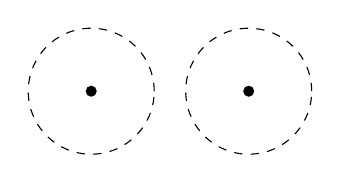
\begin{tikzpicture}[scale=1]
    % pontos
    \fill (0,0) circle (2pt);
    \fill (2,0) circle (2pt);
    % círculos tracejados sem interseção
    \draw[dashed] (0,0) circle (0.8);
    \draw[dashed] (2,0) circle (0.8);
  \end{tikzpicture}
  }
  \end{minipage} \hfill
  
\end{center}

\vspace{1.5em}



%%% T_3 %%%
\begin{center}
  \begin{minipage}{0.27\linewidth}
  \boxedpic{T$_3$}{
  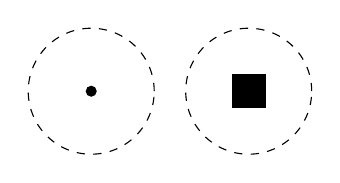
\begin{tikzpicture}[scale=1]
    % primeiro ponto
    \fill (0,0) circle (2pt);
    \draw[dashed] (0,0) circle (0.8);
    % segundo: retângulo preto
    \node[draw, fill=black, minimum width=12pt, minimum height=12pt] (R) at (2,0) {};
    \draw[dashed] (R) circle (0.8);

  \end{tikzpicture}
  }
  \begin{center}
      
  Regular $ = T_3+T_1$
  \end{center}
  
  \end{minipage} 
  \vline
  \begin{minipage}{0.27\linewidth}
    \boxedpic{T$_{3.5}$}{
  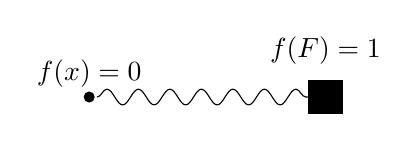
\begin{tikzpicture}[scale=1]
    % ponto com rótulo f(x)=0
    \fill (0,0) circle (2pt) node[above] {$f(x)=0$};
    % retângulo preto com rótulo f(F)=1
    \node[draw, fill=black, minimum width=12pt, minimum height=12pt] (R) at (3,0) {};
    \node at (R.north) [above=2pt] {$f(F)=1$};
    % onda ligando ponto ao retângulo
    \draw[decorate, decoration={snake, amplitude=1mm, segment length=4mm}]
      (0.1,0) -- (2.9,0);
  \end{tikzpicture}
  }
   \begin{center}
      
  Completamente Regular $ = T_{3.5}+T_1$
  \end{center}
  \end{minipage} \vline
  \begin{minipage}{0.27\linewidth}
      
    \boxedpic{T$_4$}{
  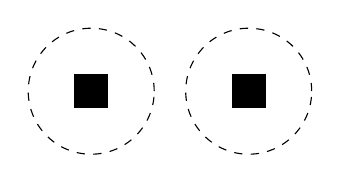
\begin{tikzpicture}[scale=1]
    % dois retângulos pretos
    \node[draw, fill=black, minimum width=12pt, minimum height=12pt] (A) at (0,0) {};
    \node[draw, fill=black, minimum width=12pt, minimum height=12pt] (B) at (2,0) {};
    % círculos tracejados sem interseção
    \draw[dashed] (A) circle (0.8);
    \draw[dashed] (B) circle (0.8);
  \end{tikzpicture}
  }
    \begin{center}
      
  Normal $ = T_4+T_1$
  \end{center}
  \end{minipage} \hfill
  
\end{center}

\vspace{1em}

%%% T_3.5 %%%
\begin{center}

\end{center}

\vspace{1em}

%%% T_4 %%%
\begin{center}

\end{center}
\end{landscape}
\end{document}